\chapter{Setup}
\label{app:setup}
In this Appendix, we provide additional information with respect to the quantum processor and the experimental setup used for this thesis. In Fig.~\ref{fig:BF1_device_picture}, we present an optical micrograph of the four-qubit quantum processor, from which we use the first three in this thesis.

\begin{figure}[htp]
  \centering
 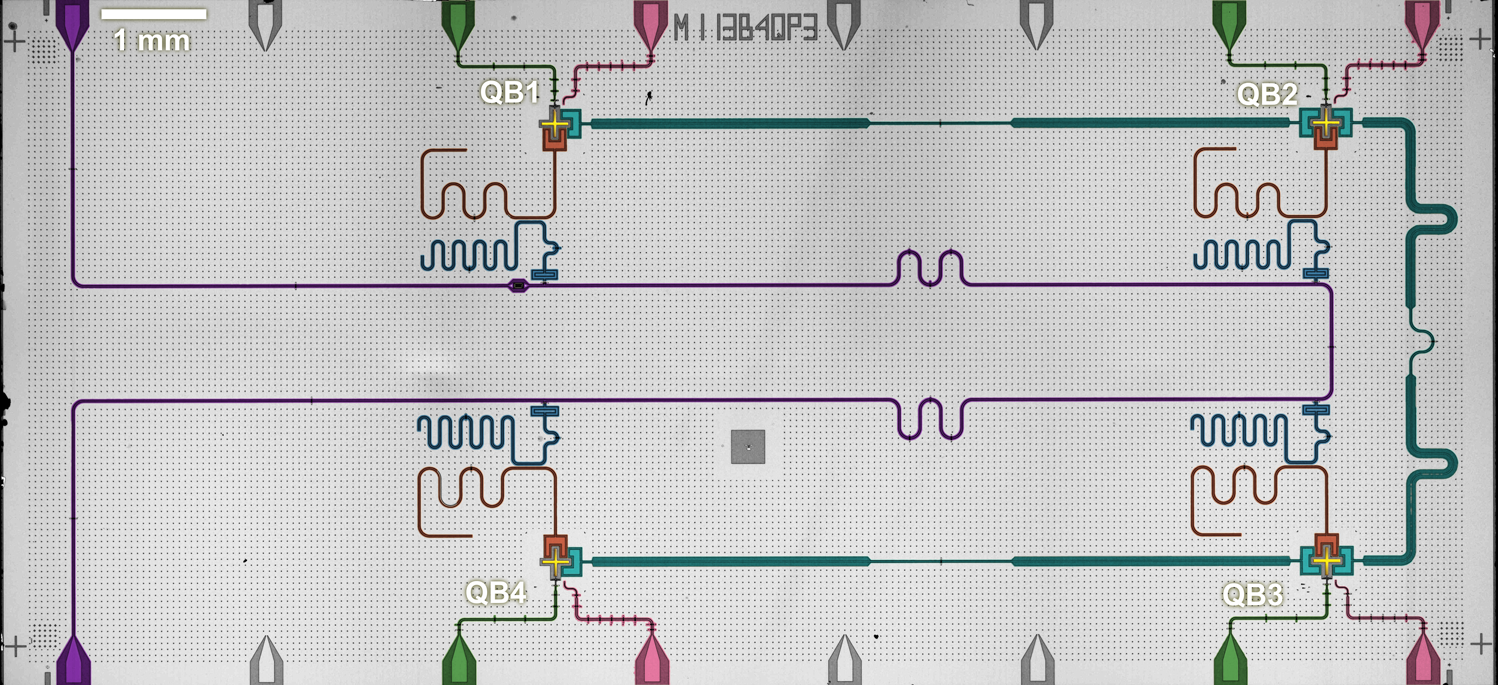
\includegraphics[width=\textwidth]{appendices/setup/figs/BF1_device.png}
 \caption{False-colored optical micrograph of the four-qubit quantum processor. The transmon qubits are colored in yellow, coupling resonators in
cyan, flux lines for single-qubit tuning in green, charge lines for single-qubit manipulation in pink, a common feedline for readout in purple,
and transmission line resonators for readout and for Purcell filtering in red and blue, respectively. Figure and caption text adapted and reproduced from Ref.~\cite{Andersen2019a}.}
 \label{fig:BF1_device_picture}
\end{figure}

In Fig.~\ref{fig:experimental_setup}, we show the detailed schematics of the the experimental setup with all relevant instruments. We use a \gls{uhf} for readout pulse generation and data acquisition, a \gls{hdawg} for single qubit pulse generation, the flux \gls{awg} for two-qubit gate flux pulses generation and a trigger \gls{awg} to synchronize all instruments. The readout line consists of a traveling-wave parametric amplifier (TWPA), a high-electron-mobility transistor (HEMT) amplifier, and the warm amplifier board (WAMP). The filters and attenuators are indicated at each temperature stage of the cryogenic system.

\begin{figure}[htp]
  \centering
 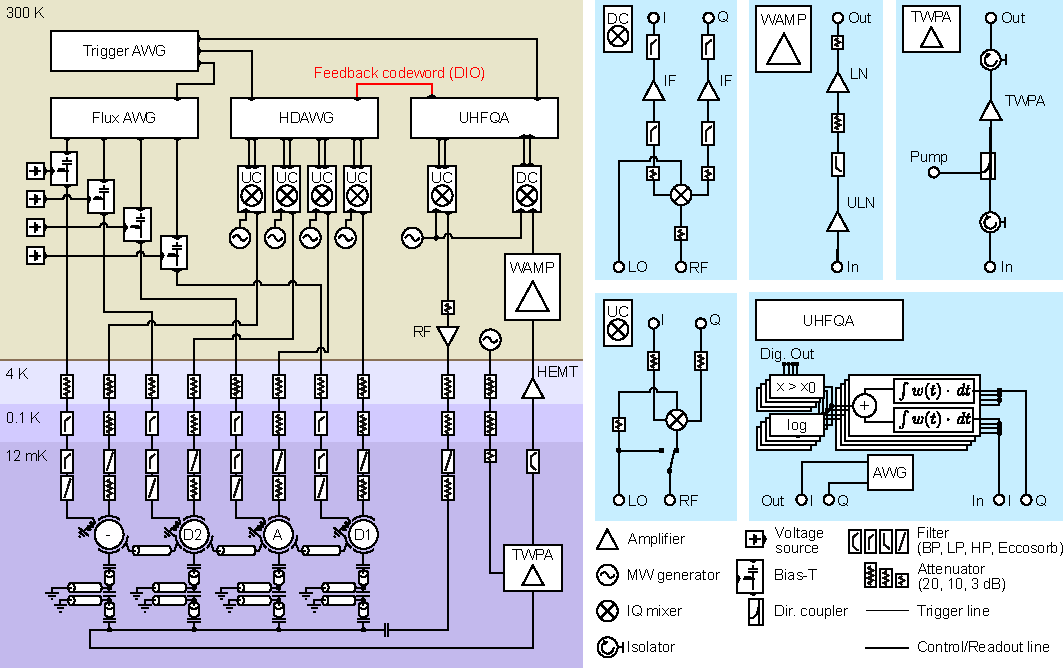
\includegraphics[width=\textwidth]{appendices/setup/figs/setup.pdf}
 \caption{Detailed schematics of the experimental setup. The filtering of the input and output signals including low-pass (LP), band-pass (BP) and infrared-blocking Eccosorb filters and attenuators are shown at the indicated temperature stages.
Extended schematics of the components of the readout chain are shown in the light blue panels. The readout signal is amplified using a traveling-wave parametric amplifier (TWPA), a high-electron-mobility transistor (HEMT) amplifier, and the warm amplifier board (WAMP) consisting of an ultra-low-noise (ULN) amplifier, a low-noise (LN) amplifier and a high-pass (HP) filter. The \gls{uhf} supports weighted integration, data logging (log) and thresholding ($x > x0$) of the readout signal. Figure and caption text reproduced and adapted from Ref.~\cite{Andersen2019}}
 \label{fig:experimental_setup}
\end{figure}

In Table~\ref{tab:app_setup_qubit_params}, we report the qubit parameters including coherence times, thermal populations and 3-level readout correct assignment probability extracted as detailed in Appendix~\ref{ch:qutrit_readout}.

\begin{table}[ht]
\centering
\caption{Coherence, frequency, coupling, and readout properties of the three qubit used in this thesis. The $T_1$ and $T_2$ times are measured at the maximum qubit frequency for qubit 1, and at the minimum qubit frequency for qubits 3. Qubit 2 is not tunable. RO stands for readout. Parameters followed by an asterisk (*) are reproduced from Ref.\  \cite{Andersen2019a}. See Ref.\ \cite{Andersen2019} for multiplexed readout.} % coherence times taken from timestamp 20191129_135651
\label{tab:app_setup_qubit_params}
\begin{tabularx}{\textwidth}{llll}
\toprule
Parameter & \textbf{Q1} & \textbf{Q2} & \textbf{Q3} \\ 
\midrule
Maximum qubit frequency* (GHz) & \multicolumn{1}{c}{5.721} & \multicolumn{1}{c}{5.210} & \multicolumn{1}{c}{5.530} \\
Minimum qubit frequency* (GHz) & 5.083 & 4.880 & 4.386  \\
Qubit lifetime ($\mu$s) & 27.8 & 16.3 & 22.9  \\
Qubit Ramsey coherence time ($\mu$s) & 25.4 & 20.0 & 12.5  \\
Qubit echo coherence time ($\mu$s) & 32.4 & 22.8 & 22.4 \\
Readout resonator frequency (GHz) & 6.890 & 7.085 & 6.686  \\
Purcell resonator – RO resonator detuning* (MHz) & 29.5 & 27.5 & 19.4 \\
Purcell resonator – RO resonator coupling* (MHz) & 10.9 & 8.2 & 9.5 \\
Purcell resonator to half-feedline coupling* (MHz) & 27.2 & 34.7 & 10.7 \\
Effective readout resonator linewidth* (MHz) & 2.4 & 2.0 & 1.5  \\
Dispersive shift* (MHz) & -3.9 & -1.6 & -1.8 \\
Thermal population (\%) & 0.9 & 0.4 & 1.4  \\ 
3-level RO assignment prob. (no preselection) (\%) & 97.42 & 96.57 & 95.71\\
\bottomrule
\end{tabularx}
\end{table}

In Table~\ref{tab:cz_gate_params}, we report the two-qubit gate parameters used for the \gls{qaoa} experiments.

\begin{table}[ht]
\centering
\caption{\gls{cz} parameters as used for \gls{qaoa}.}
\begin{tabularx}{\textwidth}{lll}
\toprule
Parameter & \textbf{Q1}-\textbf{Q2} & \textbf{Q2}-\textbf{Q3}   \\ 
\midrule
Pulse length (ns) & 94 &  107 \\
Pulse amplitude (V)  & 0.785 & 0.229  \\
Gaussian filter standard deviation (ns) & 1 & 1  \\ % note: 1 in pulse and 2 in FIR filter
Buffer before pulse (ns) & 15 & 10  \\
Buffer after pulse (ns) & 15 & 15 \\
Maximum leakage (\%) & 9 & 2.5  \\
\bottomrule
\end{tabularx}
\label{tab:cz_gate_params}
\end{table}
